\chapter{Introduction} \label{ch:intro}

\section{Context}\label{sec:context}

The continuous evolution of mobile networks, driven by an increasing number of users, devices, and online applications, has been marked by successive generations of technological advancements.
These advancements have introduced increased complexity and a growing reliance on proprietary solutions.
This reliance has restricted, the potential for open and interoperable architectures, posing issues significant challenges to the integration of new technologies.

A persistent challenge in this context is Line-of-Sight (LoS) obstruction.
LoS obstruction occurs when the direct visual path between a transmitter and receiver is impeded, often leading to signal attenuation, degradation in communications quality, or even complete loss of connectivity.
While LOS obstruction has been a concern across all generations of wireless networks, its significance has become increasingly pronounced with the use of higher frequency bands and denser network deployments characteristic of the recently released 5G and future 6G technologies.
These networks leverage millimeter-wave frequencies for data transmission, which are highly sensitive to obstacles such as buildings, foliage, and terrain irregularities, exacerbating LOS-related challenges.

Looking ahead to the 6G paradigm, it is evident that while it promises unprecedented levels of connectivity and technological innovation,  LoS obstruction will potentially become even more challenging.
The envisioned 6G networks are expected to operate at even higher frequencies to accommodate increasing demands for data transmission rates and ultra-low latency applications, such as Augmented Reality (AR) and autonomous systems.

Given these anticipated deployment and challenges, it is important to address the  LoS obstruction concern and develop solutions capable of adapting to the evolving demands of wireless communications infrastructures.
Furthermore, there is an increasing recognition of the importance of open and interoperable architectures in accelerating technological progress.
Therefore, there is a pressing need to develop open-source solutions that integrate with existing network infrastructures while accommodating future advancements.

\begin{figure}[H]
    \centering
    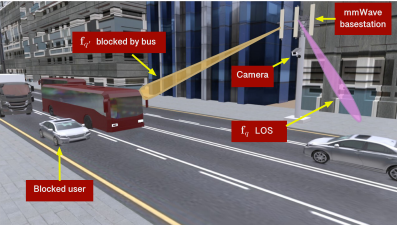
\includegraphics[width=0.7\linewidth]{figures/urban_scenario}
    \caption[mmWave base station equipped with camera to monitor LoS obstruction to users]{mmWave base station equipped with camera to monitor LoS obstruction to users \cite{Block_predict}.}
    \label{fig:urban_scenario}
\end{figure}

Within 6G, integrating mobile Base Stations (BSs) will be an enabler for achieving ubiquitous, network connectivity.
Radio Access Networks (RANs), consisting of mobile BSs, offer a dynamic and on-demand deployment approach, promising to meet varying Quality of Service (QoS) requirements in diverse contexts.
However, taking advantage of the full potential of mobile BSs requires developing software applications that can optimize RAN management.
In this context, leveraging xApps and rApps, defined by the O-RAN architecture, is a promising approach to optimize RANs and facilitate the integration of radio, sensing and vision-based information.

This approach paves the way for perception-aided mobile RANs, where real-time environmental awareness can overcome challenges in signal propagation and locating mobile devices that seek wireless connectivity.
In this context, Computer Vision (CV) is expected to enhance networks with capabilities beyond traditional telecommunications systems.
Using multiple sensors and video cameras, real-time environmental awareness may become a cornerstone for network optimization.
For that purpose, state-of-the-art CV algorithms may take charge of tasks related to processing and interpreting visual data while proactively identifying obstacles to prevent signal attenuation and blockage.
This convergence of CV and communications represents a promising advancement, holding the potential for improved heightened responsiveness, adaptability, and overall network performance.

\section{Motivation and Problem}\label{sec:motivation-and-problem}

In the ongoing evolution of mobile networks, successive generations have expanded connectivity capabilities while introducing heightened complexity.
This complexity, along with a growing dependence on closed, proprietary solutions, represents a significant challenge to integrating diverse technologies.
Recognizing these limitations is crucial, leading to the emergence of the 6G paradigm as a revolutionary response.
This paradigm envisions an evolution from closed systems to open-source implementations with open interfaces, where mobile networks complexity is managed through interoperable solutions.
The 6G paradigm stands as a catalyst for change in wireless communications.

However, the 6G paradigm faces a new layer of complexity due to dynamic and moving obstacles,  which can compromise communications in high-frequency bands.
This complexity arises the shorter wavelengths, making signals more prone to attenuation when encountering obstacles.
Millimeter-wave signals struggle to penetrate solid structures such as walls and buildings, potentially causing signal blockages and coverage gaps in densely populated urban areas.
The presence of vehicular traffic, pedestrians, and other mobile entities in the network's coverage area creates ephemeral shadowing effects, leading to signal blockages and fluctuations that directly impact wireless connectivity reliability.
This dynamism poses a considerable challenge to maintaining consistent signal strength and QoS levels, especially in areas with high vehicular or pedestrian density.
Addressing the dynamic nature of signal attenuation introduced by moving obstacles requires adaptive solutions, advanced signal tracking, predictive algorithms, and real-time adjustments in network configuration.

Furthermore, the distinction between LoS and Non-Line-of-Sight (NLoS) propagation paths adds to the challenge.
LOS paths, with a direct, unobstructed line between the transmitter and receiver, typically offer the most reliable and efficient communications.
However, in urban environments, NLoS paths, where signals reflect off buildings or scatter due to obstacles, become prevalent.
These NLoS paths introduce additional challenges, such as multipath fading and increased signal attenuation, further exacerbating connectivity issues.

A promising solution to the wireless communications challenges faced in densely populated urban areas lies in obstacle-aware networks, that leverage CV to extract information from video data.
By integrating CV algorithms, wireless networks can recognize and proactively overcome the challenges posed by moving obstacles.
This approach holds the potential to ensure uninterrupted communications and foster a seamless network experience in urban environments, aligning with the vision set forth by the 6G paradigm.

\section{Objectives}\label{sec:objectives}

The main objective of this dissertation was to implement vision-based RAN. This solution provides a Base Station to with environmental real-time perception provided by vision-based information.

In order to achieve this goal, specific objectives were defined:

    \begin{itemize}
    
    \item Implement a mechanism for detecting and tracking objects within the gNB's operational environment, enhancing the gNB's ability to adapt to dynamic environments.
    
    \item Develop a solution that extracts relevant information from video, through Computer Vision.
    This solution should provide information to the mobile network in real time to enhance the gNB's perception and obstacle awareness capabilities.
    
    \item Create a set of messages with information inferred from real-time video.
    This set should be relevant in the context of mobile networks, particularly for use by the gNB\@.
    These messages should be compliant with the O-RAN architecture.
    
    \item Develop an algorithm, implemented as an xApp, capable of receiving video-extracted information and RAN metrics to provide environmental perception for a RAN node.
      
    \item Validate and evaluate the proposed solution in reference networking scenarios.
    
    \end{itemize}

\section{Contributions}\label{sec:contributions}

The main contributions are the following:

    \begin{itemize}
    
    \item The introduction of video-based information into a 5G network, based on O-RAN architecture.
    This solution extracts relevant information from video feeds, tailored to indoor 5G use case.
    This is possible due to the development of a set of structured messages containing video-extracted information.
    These messages are specifically designed for improving network performance and obstacle management of the gNB\@.
    
    \item A xApp that processes video-extracted information and RAN metrics to determine optimal placement and configuration for a RAN\@.
    This application enhances the gNB's capabilities by enabling it to make informed decisions based on real-time environmental perception.
    
    \item The validation and evaluation of the performance of the proposed solution in a reference networking scenario.
    This includes a proof-of-concept for evaluating vision-aided networking solutions.
    
    \end{itemize}


% adjust references to chapters
\section{Document Structure}\label{sec:document-structure}

This document follows a structured approach.
Chapter~\ref{ch:state-of-the-art} discusses state-of-the-art and related work, addressing concepts related with to the challenges tackled in this dissertation.
Chapter~\ref{ch:specs_design_implem} outlines the proposed solution, detailing the system's specifications, design choices, and implementation.
Chapter~\ref{ch:validation} presents the experimental tests conducted to validate and evaluate the implementation of the proposed solution.
Finally, Chapter~\ref{ch:conclusion} synthesizes findings, draws conclusions, and provides directions for future work.